\pagenumbering{arabic}
\Large
% \normalsize
\label{Chapter_1}

Data sharing has become a foundational enabler of modern industry, research, and
governance, driving collaborative decision-making, operational efficiency, and
innovation across organisational boundaries. Its economic weight is now
substantial: the OECD estimates that data sharing could contribute on the order
of 2.5\% of global GDP~\cite{oecd2019data}, and regulatory instruments such as
the EU Data Act of 2023 reflect a growing recognition of its strategic
importance~\cite{eu2023dataact}.
Within this landscape, the Industrial Internet of Things (IIoT) has emerged as a
core substrate: heterogeneous sensors, programmable logic controllers,
actuators, and edge nodes are interconnected to support real-time data
collection, autonomous decision-making, and adaptive control across
manufacturing, energy, water, and transportation infrastructure.
 
The scale of this connectivity is now infrastructure-sized. The global installed
base of connected IoT devices reached approximately 18.5~billion in 2024, was
projected to reach 21.1~billion by the end of 2025, and is forecast to reach 39~billion by 2030,
a compound annual growth rate of about 13.2\%~\cite{iotanalytics2025}. As
industrial operations become increasingly dependent on continuous
machine-to-machine exchange, the authenticity, timeliness, and confidentiality
of that data cease to be optional and become operationally critical.
 
This dependence is precisely what elevates IIoT security to a first-order
concern. Pervasive connectivity substantially expands the attack surface and
exposes industrial infrastructure to sophisticated threats, including zero-day
attacks that evade conventional detection~\cite{amadi2026lightweight}. The threat
landscape has responded in kind. Operational-technology (OT) environments have
become mainstream targets: ransomware activity against industrial organisations
rose by 87\% year over year, the number of ransomware groups targeting
such organisations grew by 60\% to reach 80, and manufacturing alone accounted
for more than half of observed victims; roughly one quarter of these incidents
forced a full shutdown of the affected OT site~\cite{dragos2025}. The financial
consequences are comparable in magnitude, with the global average cost of a data
breach reaching USD~4.44~million and rising to USD~10.22~million in the United
States~\cite{ibm2025}. Fig.~\ref{fig:landscape} summarises these indicators.
These figures establish the stakes; the difficulty, however, lies in which
devices must bear the security burden.

\begin{figure}[htbp]
    \centering
    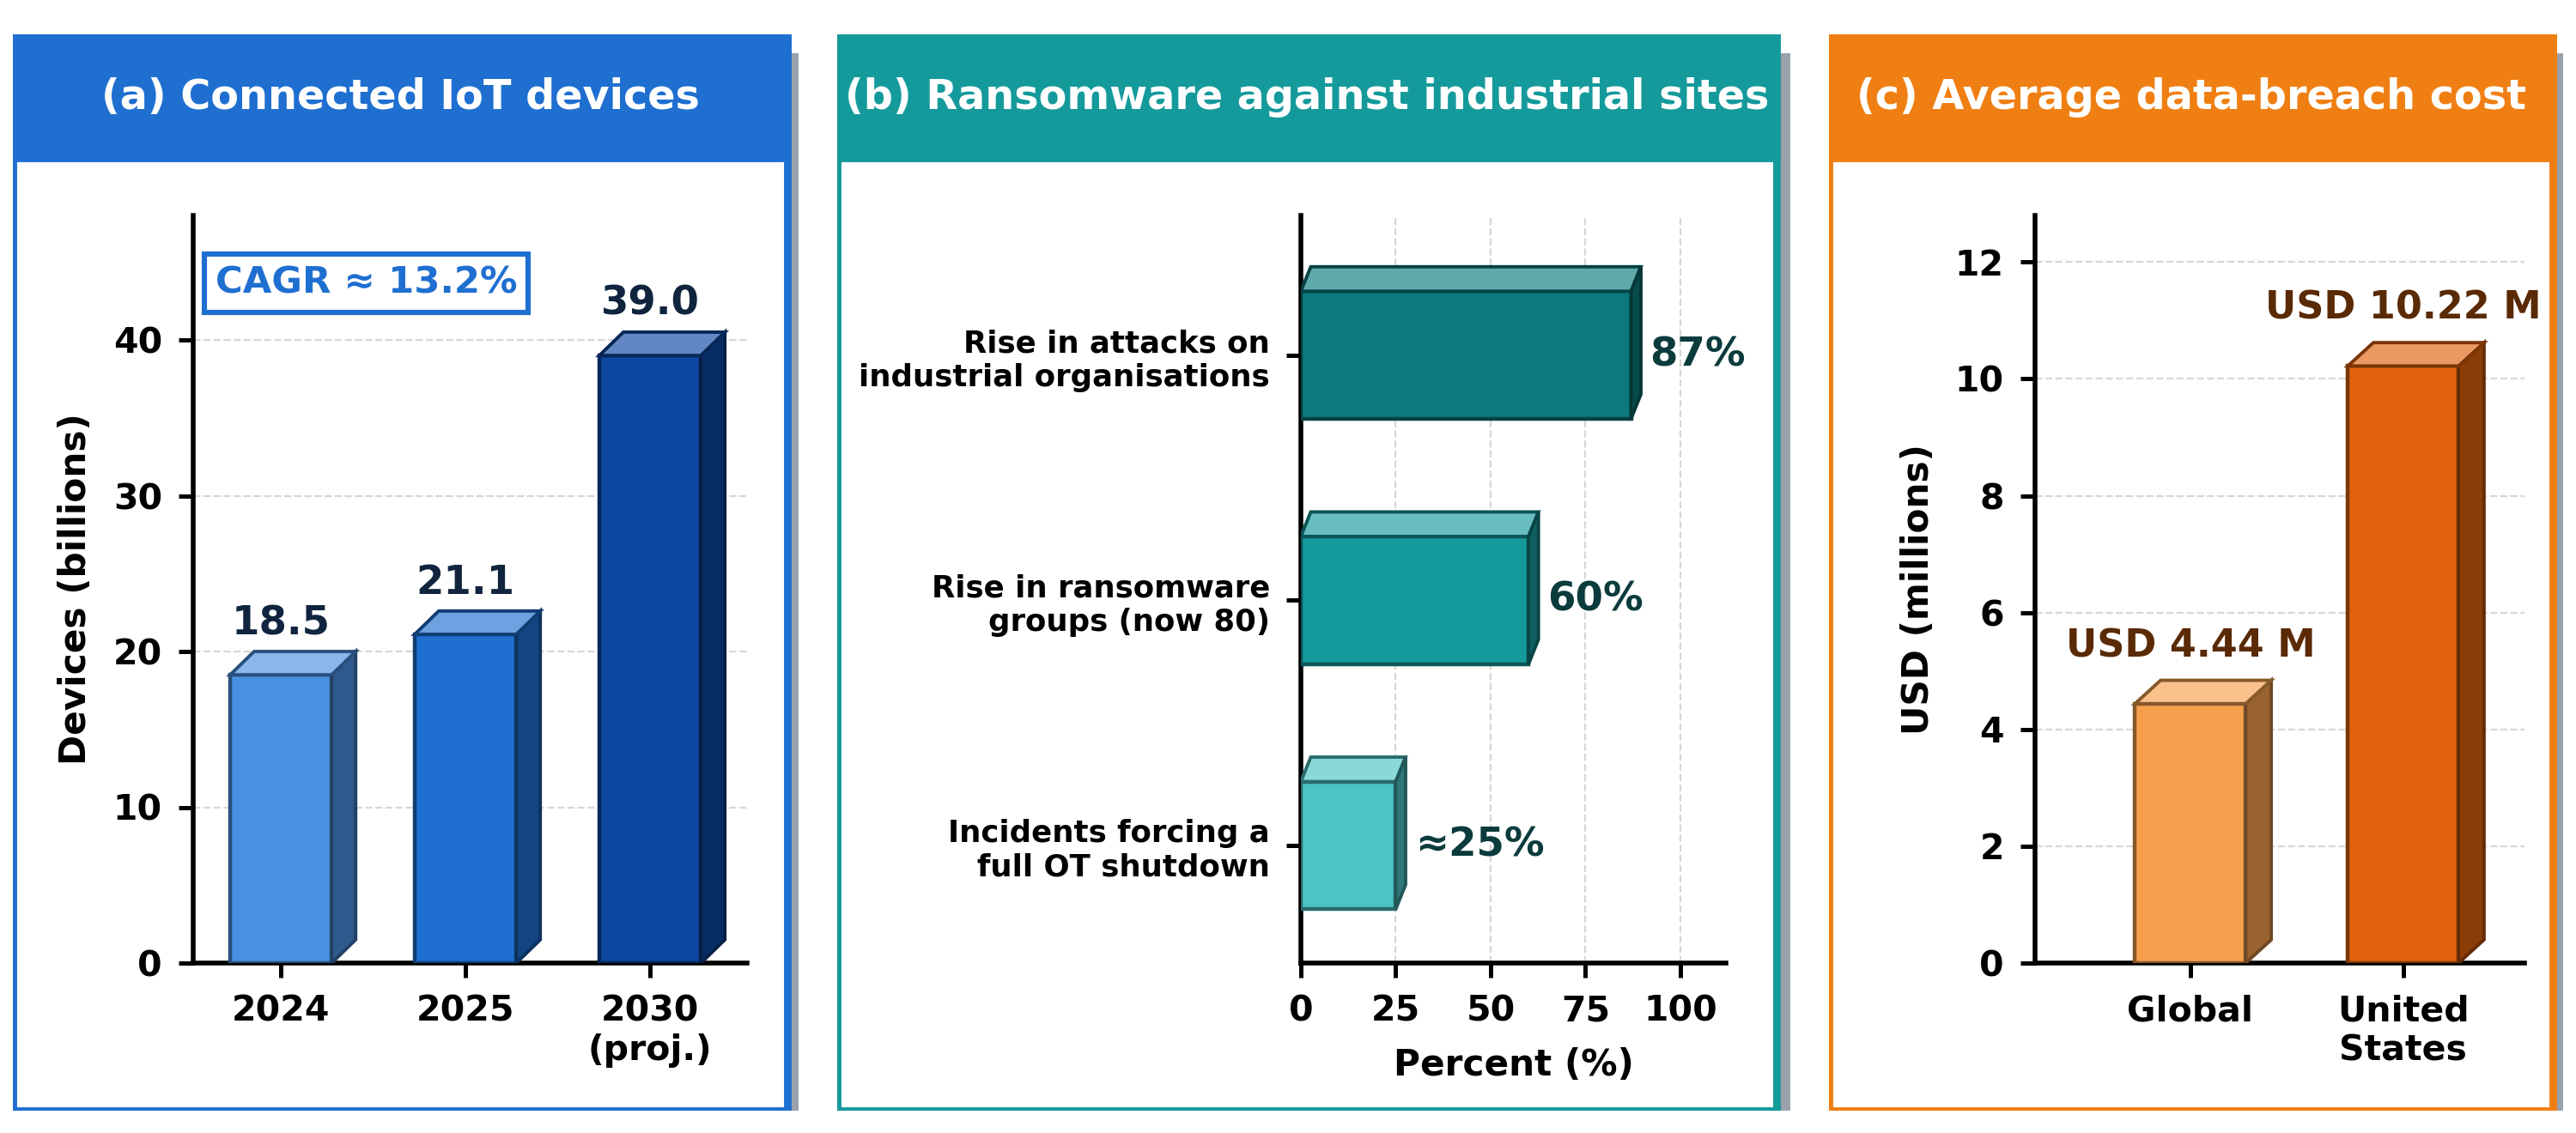
\includegraphics[width=\textwidth]{figures/Fig1_2_landscape.png}
    \caption{Indicators of the IIoT security landscape: (a) growth of connected IoT devices from 2024 to 2030~\cite{iotanalytics2025}; (b) ransomware activity against industrial organisations~\cite{dragos2025}; and (c) the average cost of a data breach globally and in the United States~\cite{ibm2025}.}
    \label{fig:landscape}
\end{figure}
 
The nodes at the edge of an IIoT deployment are severely resource-constrained,
operating within tight budgets of computation, memory, and energy. These
constraints hinder the deployment of conventional deep learning-based intrusion
detection and heavyweight cryptographic machinery on the very devices that most
require protection~\cite{amadi2026lightweight}. The central engineering tension of
secure IIoT is therefore not whether strong protection exists, but whether it
can be delivered within the resource envelope of constrained devices without
sacrificing the real-time responsiveness that mission-critical operations
demand.
 
Distributed ledgers are a natural foundation for tamper-evident trust among such
devices, yet they bring a constraint of their own. This tension is a concrete
instance of the well-documented blockchain trilemma: the difficulty of
simultaneously achieving security, scalability, and speed
within a single distributed-ledger system, where optimising any two dimensions
tends to come at the expense of the third~\cite{aiv_own}. Recent theoretical
work argues that these trade-offs are not merely engineering compromises but
reflect fundamental limits, supported by formal proofs of their
inevitability~\cite{nakai, mssassi, monte}. In safety-critical,
resource-constrained settings the trilemma is at its most acute, since none of
the three dimensions can be relaxed without unacceptable consequence.
 
A further pressure compounds the problem. The asymmetric cryptography that
underpins current authentication and key exchange, namely RSA and
elliptic-curve schemes, is vulnerable to a sufficiently capable quantum computer executing
Shor's algorithm~\cite{shor1999polynomial}. The risk is not deferred to the
arrival of such a machine: under the ``harvest-now, decrypt-later'' model, an
adversary can capture encrypted traffic today and decrypt it retroactively once
the capability matures, placing data with long confidentiality horizons at
present risk~\cite{kagai2025harvest}. This
concern is now codified rather than speculative. In August 2024, the U.S.
National Institute of Standards and Technology finalised its first
post-quantum cryptographic standards, FIPS~203 (ML-KEM, derived from
CRYSTALS-Kyber), FIPS~204 (ML-DSA), and FIPS~205 (SLH-DSA), concluding a
standardisation process initiated in 2016~\cite{fips203, fips204, fips205}. For
constrained IIoT the challenge is sharper still, as post-quantum primitives
carry larger keys and ciphertexts than the schemes they replace and must be made
to fit hardware already strained by classical cryptography.

\begin{figure}[htbp]
    \centering
    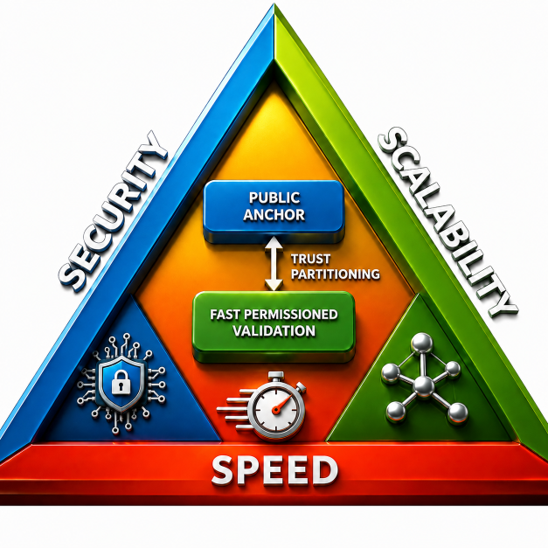
\includegraphics[width=0.70\textwidth]{figures/Picture1.png}
    \caption{The security, scalability, and speed trilemma in constrained mission-critical IIoT, and the trust-partitioning response adopted in this thesis, in which fast permissioned validation is separated from public anchoring.}
    \label{trilemma}
\end{figure}

Several approaches have been proposed to meet these pressures, but each resolves
one at the expense of another. Learning-based detectors built on convolutional,
recurrent, and hybrid convolutional-recurrent models achieve strong accuracy on
industrial traffic~\cite{chen2025cnnlstm, anwer2025federated}, and federated
variants keep raw data on the premises that generate
it~\cite{lee2025lightweight, mao2025fedinnid}. However, the trust verdict these
detectors produce is stored wherever the model runs, so it remains as mutable as
its host. Permissioned ledgers coupled to intrusion detection make such verdicts
tamper-evident~\cite{song2025hybrid, peng2025bctdics}, yet committing at
industrial event rates strains consensus throughput and on-chain
storage~\cite{xiong2025sharding, ding2025dcstorage}. Hybrid and tiered ledgers
reconcile operational speed with external verifiability by anchoring a compact
digest of a fast permissioned layer on a public
chain~\cite{ullah2025mbid, banitalebi2025edblsd}. In doing so, however, they make
the cross-chain link the weakest point of the combined
system~\cite{zhou2025bridgeguard}, and the quantum-resistant primitives needed
to keep the anchored record durable carry keys and signatures that collide with
the budgets of constrained devices~\cite{hanna2025comprehensive, cruz2025measuring}.
What is required is therefore not a stronger single layer of protection, but a
design that places each security function where its cost can be sustained.
 
Taken together, these forces define the gap this thesis addresses. Trustworthy
IIoT security must be affordable within real device resource budgets, responsive
enough for mission-critical operation, scalable across large deployments, and
resilient against an emerging quantum adversary, a combination that a single,
uniform security layer cannot satisfy simultaneously. The position advanced in this thesis is that these demands become jointly achievable when trust is not
applied uniformly but is partitioned across a tiered architecture:
high-frequency behavioural validation is routed through a fast, permissioned
layer close to the devices, while low-frequency, high-value events such as
identity anchoring, audit, and revocation are committed to a separate public
layer, as illustrated in Fig.~\ref{trilemma}. Routing sensitive,
high-frequency interactions through permissioned consensus while anchoring
integrity proofs and audit trails on public chains has been argued to be a
structural necessity rather than a mere performance optimisation for demanding
data-sharing environments~\cite{amadi2026security}. This principle of trust-partitioning across a hybrid
ledger, and its realisation within real device budgets and across distinct
ledger substrates, forms the central contribution of this thesis.


\section{Motivation for Research}
\label{motivation}

This study is motivated by the gap between the security that mission-critical
IIoT requires and the security that constrained industrial hardware can afford.
Existing approaches tend to optimise one dimension at the expense of the others.
Many intrusion-detection methods pursue model accuracy without demonstrating
that the model, together with its supporting ledger, can run on a low-power node;
many blockchain provenance schemes secure storage without establishing
feasibility on constrained devices; and most report neither a complete
evaluation across both the artificial-intelligence and blockchain layers nor the
blockchain-side costs, such as gas consumption, transaction latency, and
smart-contract security, that determine real-world viability. At the same time,
the reliance on classical asymmetric cryptography leaves long-lived industrial
data exposed to a quantum adversary under the harvest-now, decrypt-later model,
a concern now formalised by the standardisation of post-quantum algorithms.
Rather than treating efficiency, security, and quantum resilience as competing
objectives to be traded against one another, this research is driven by the view
that they can be reconciled by disaggregating trust across a tiered architecture,
so that each security function is placed on the layer whose cost profile it can
sustain. The aim is a security design that is lightweight, verifiable, and
deployable on real industrial devices, and whose organising principle
generalises beyond any single implementation.

\section{Research Breakdown and Major Contributions}
\label{sec:rq}

The foregoing analysis exposes a single overarching problem. How can trustworthy
security be delivered for constrained, mission-critical IIoT when the devices
that carry the security burden cannot afford uniform, heavyweight protection,
and when the underlying cryptography faces an emerging quantum threat? From this
problem, the following research questions follow:

\begin{enumerate}
  \item \textbf{Trust partitioning:} Can trust be partitioned across a hybrid
        ledger, so that high-frequency behavioural validation is handled on a
        fast permissioned layer while low-frequency, high-value events such as
        identity anchoring, audit, and revocation are committed to a separate
        anchoring layer, and does this partitioning deliver trustworthy security
        within real device resource budgets?

  \item \textbf{Lightweight behavioural trust:} Can lightweight
        artificial-intelligence behavioural trust scoring operate inside the
        compute, memory, and energy budgets of real constrained IIoT devices
        without sacrificing detection performance?

  \item \textbf{Quantum-resilient identity:} Can post-quantum-resilient identity
        and credential delivery be achieved on such hardware without prohibitive
        latency or bandwidth cost?

  \item \textbf{Substrate independence:} Does the trust-partitioning principle
        hold across distinct ledger substrates, rather than being an artefact of
        a single implementation?

  \item \textbf{Adversarial robustness:} Under adversarial conditions, can
        behavioural trust scoring with decay-based revocation reliably isolate a
        misbehaving node while the hybrid-ledger architecture sustains
        dependable detection performance?
\end{enumerate}

Answering these questions requires an architecture that reconciles scalability
with speed and security while carrying out validation and anchoring within the
resource limits of industrial edge hardware. The goal of this thesis is
therefore to establish that trustworthy security for constrained,
mission-critical IIoT is achievable by partitioning trust across a hybrid-ledger
architecture, in which high-frequency behavioural validation is handled on a
fast permissioned layer and low-frequency, high-value events are anchored on a
public layer, and to demonstrate this within real device resource budgets and
across more than one ledger substrate. Toward this goal, this research makes the
following contributions:

\begin{enumerate}
  \item It introduces STRATA, a unified trust-partitioning architecture for
        constrained, mission-critical IIoT, in which high-frequency behavioural
        validation on a fast permissioned layer is separated from low-frequency
        identity anchoring and audit committed to a public layer, and it
        consolidates three published
        systems~\cite{amadi2026lightweight, amadi2025quantum, amadi2026symmetric}
        as instances of this single architecture rather than as independent
        designs.

  \item It presents a lightweight federated behavioural-trust module built on a
        trimmed one-dimensional CNN-LSTM model coupled with a resource-optimised
        permissioned ledger, and evaluates it end to end across both the
        artificial-intelligence and blockchain layers, reporting detection
        performance together with blockchain-side
        costs~\cite{amadi2026lightweight}.

  \item It presents a quantum-resilient identity and credential module based on
        entropy-seeded identity generation and compressed post-quantum key
        delivery, and demonstrates its feasibility on constrained hardware,
        distinguishing clearly between the components that are implemented and
        measured and those reserved as design~\cite{amadi2025quantum}.

  \item It demonstrates that the trust-partitioning principle is
        substrate-independent by realising it on two distinct ledger
        substrates~\cite{amadi2026lightweight, amadi2026symmetric}, and it provides a consolidated evaluation, spanning
        detection performance, resource overhead, blockchain cost, and
        quantum-resilience, that assesses the architecture against the resource
        constraints of industrial edge devices.
\end{enumerate}

The systematic review in Chapter~3 found no prior work that establishes trust
partitioning across a hybrid ledger as a unifying principle for constrained,
mission-critical IIoT, demonstrated within real device budgets and shown to hold
across distinct ledger substrates. This constitutes the novelty of the thesis.

Table~\ref{tab:rq-map} maps each research question to the contribution that
answers it, the sections in which it is designed and evaluated, and the
published work on which it builds.
\begin{table}[htbp]
\centering
\footnotesize
\setlength{\tabcolsep}{4pt}
\renewcommand{\arraystretch}{1.35}
\caption{Mapping of the research questions to the contributions, the thesis sections that design and evaluate them, and the underlying publications.}
\label{tab:rq-map}
\begin{tabularx}{\textwidth}{@{}
    >{\raggedright\arraybackslash}p{0.9cm}
    >{\raggedright\arraybackslash}X
    >{\centering\arraybackslash}p{1.3cm}
    >{\raggedright\arraybackslash}p{2.1cm}
    >{\raggedright\arraybackslash}p{2.4cm}
    >{\raggedright\arraybackslash}p{2.2cm}@{}}
\toprule
\textbf{RQ} & \textbf{Focus} & \textbf{Contri\-bution} & \textbf{Design (Ch.~4)} & \textbf{Evaluation (Ch.~5)} & \textbf{Publication} \\
\midrule
RQ1 & Partitioning trust across a hybrid ledger within device budgets
    & 1 & \ref{sec:strata-principle}, \ref{sec:strata-anchor}
    & \ref{sec:eval-ledger}, \ref{sec:eval-trilemma}
    & \cite{amadi2026security, amadi2026lightweight} \\
RQ2 & Lightweight behavioural trust scoring on constrained devices
    & 2 & \ref{sec:strata-trust}
    & \ref{sec:eval-evidence}, \ref{sec:eval-learning}, \ref{sec:eval-resource}
    & \cite{amadi2026lightweight} \\
RQ3 & Quantum-resilient identity and credential delivery
    & 3 & \ref{sec:plane-b}
    & \ref{sec:eval-identity}
    & \cite{amadi2025quantum, amadi2026symmetric} \\
RQ4 & Substrate independence of trust partitioning
    & 4 & \ref{sec:strata-substrates}
    & \ref{sec:eval-substrate}
    & \cite{amadi2026lightweight, amadi2026symmetric} \\
RQ5 & Isolating a misbehaving node under adversarial conditions
    & 2, 3 & \ref{sec:plane-a}
    & \ref{sec:eval-security}, \ref{sec:eval-isolation}
    & \cite{amadi2026symmetric} \\
\bottomrule
\multicolumn{6}{@{}p{\textwidth}@{}}{\scriptsize The trilemma framing of Chapters~1 and~2 draws on~\cite{aiv_own}, and the systematic review of Chapter~3 extends~\cite{amadi2026security}.}
\end{tabularx}
\end{table}

\label{sec:organisation}
The organisation of this thesis is as follows. Chapter~\ref{Chapter_1}
presents the introduction, the motivation, the research questions, and the
contributions. Chapter~2 provides the background, covering consensus and hybrid
ledgers, post-quantum cryptography, and lightweight learning for anomaly
detection. Chapter~3 reviews related work and, through a systematic analysis,
identifies the defence gap that the thesis addresses. Chapter~4 presents the
STRATA architecture and its constituent modules as instances of a single
trust-partitioning design. Chapter~5 reports the consolidated evaluation across
detection performance, resource overhead, blockchain cost, and quantum
resilience. The thesis is concluded in Chapter~6 with a summary of
contributions, the disclosed limitations, and directions for future work.
Fig.~\ref{fig:roadmap} presents this structure as a roadmap, indicating the
research questions each chapter addresses.

\begin{figure}[htbp]
    \centering
    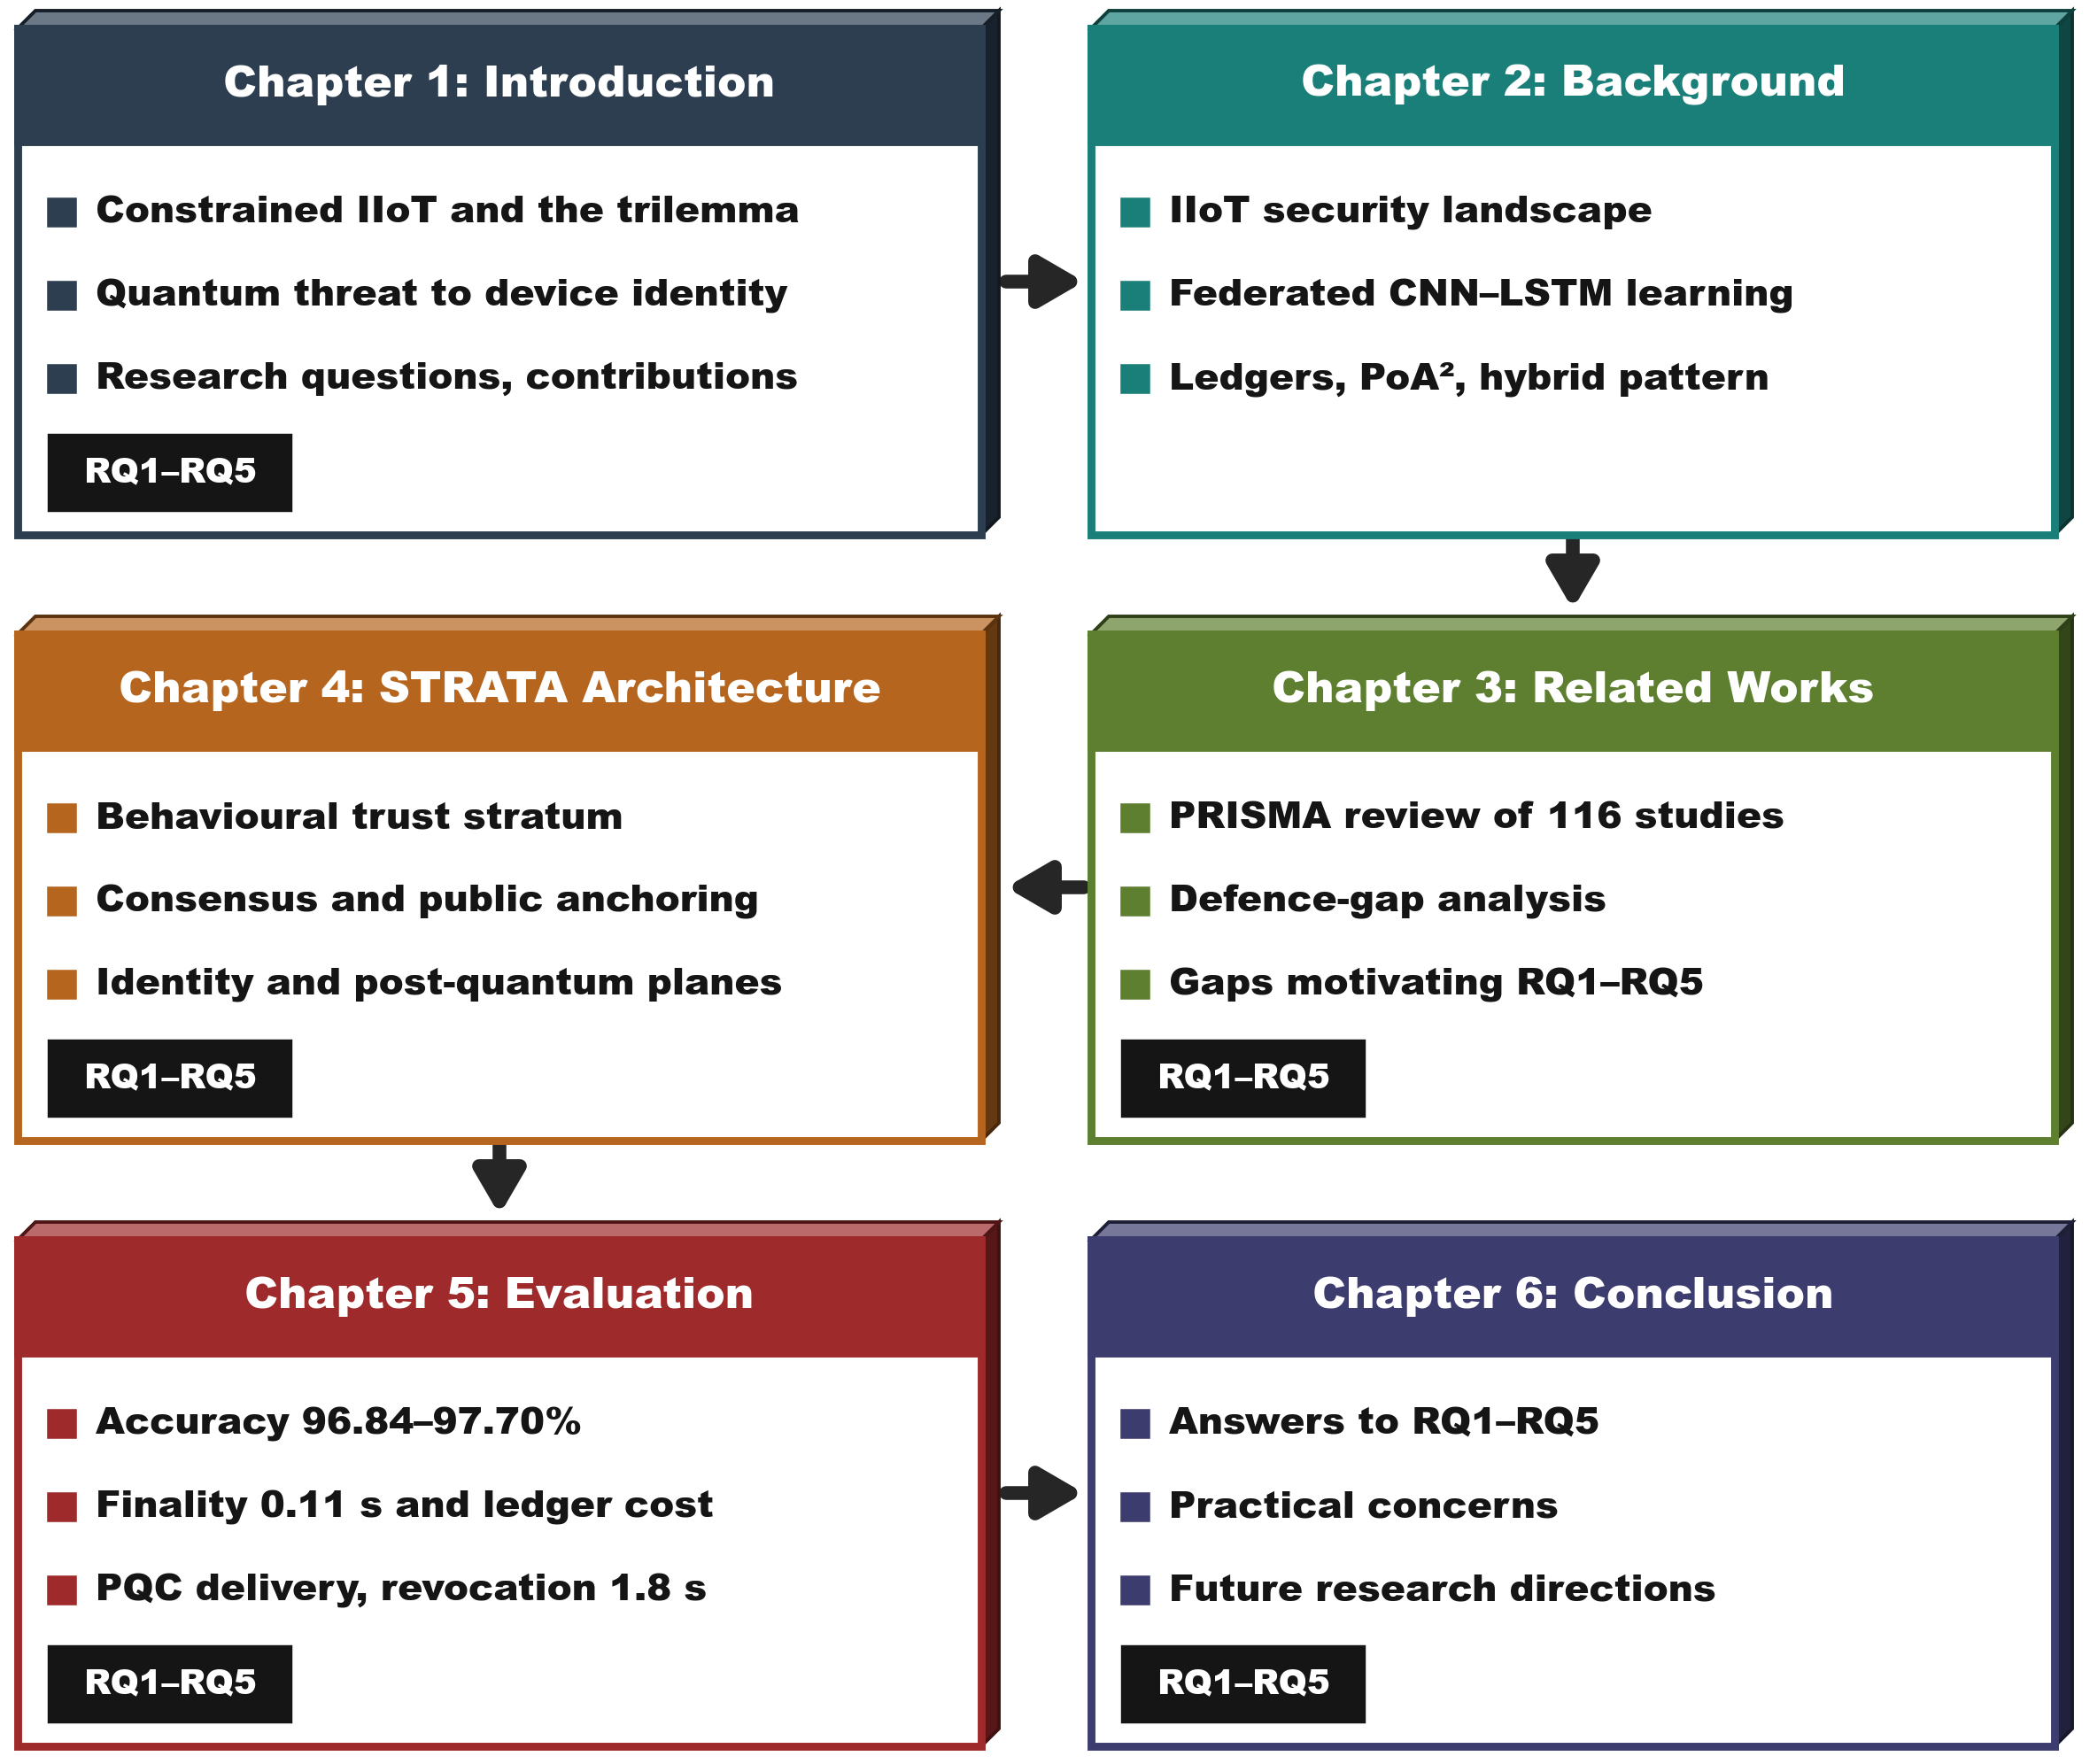
\includegraphics[width=\textwidth]{figures/Fig1_3_roadmap.png}
    \caption{Roadmap of the thesis, showing the flow from problem definition to the STRATA architecture, its evaluation, and the conclusions, together with the research questions associated with each chapter.}
    \label{fig:roadmap}
\end{figure}
